%=====================
\chapter{Requirements}
%=====================
\label{chap:req:requirements}
This chapter describes a \gls{utility} that creates \Gls{wireshark} \glspl{dissector} from \Gls{c}
\gls{header} files. The \glspl{dissector} must interpret \gls{binary} representations of \Gls{c}
\glspl{struct}. In \autoref{sec:req:list} we give a high level overview of the
\gls{utility} and lists all the functional and non-functional requirements, 
while \autoref{sec:req:usecases} provides use cases for the \gls{utility}, 
and \autoref{sec:prodbacklog} contains the complete product backlog.


%-----------------------------
\section{List of Requirements}
%-----------------------------
\label{sec:req:list}
We are to create a \gls{utility} that allows \Gls{wireshark} to interpret the \gls{binary}
representations of \Gls{c}-language \glspl{struct}. While \Gls{c} \glspl{struct} seldom are exchanged
across networks, they are sometimes used in \gls{ipc}. The
purpose of the \gls{utility} described here is to provide \Gls{wireshark} with the
capability of automatically dissecting the \gls{binary} representation of a \Gls{c} \gls{struct},
as long as its definition is known.

The expected work flow for the \gls{utility} is to read one or more \Gls{c} \gls{header} files,
which contain \gls{struct} definitions, and output \Gls{wireshark} \glspl{dissector}, implemented
in \Gls{lua} scripts. A configuration file or source code annotations in the \gls{header}
files may be used when additional configuration is required.

\autoref{tab:req:func} and \autoref{tab:req:func2} lists the functional requirements,
while \autoref{tab:req:nonfunc} lists non-functional requirements.
Each requirement have a priority (Pri) and a complexity (Cmp): \Gls{h}, 
\Gls{m} or \Gls{l}. This is explained in \autoref{sec:req:priority}
and \autoref{sec:req:compl}.

\subsection{Prioritization}
%--------------------------
\label{sec:req:priority}
The team has, in cooperation with the customer, prioritized the requirements
in four categories:
\begin{inparaenum}[\itshape a\upshape)]
	\item High,
	\item Medium,
	\item Low or
	\item Optional.
\end{inparaenum} 

\begin{description}
	\item[High] Core functionality of the \gls{utility} that must be implemented.
	\item[Medium] Requirements that will improve the value of the \gls{utility}.
	\item[Low] Requirements that will not add much value to the \gls{utility}.
	\item[Optional] Requirement that may be implemented depending on available time.
\end{description}

\subsection{Complexity}
%----------------------
\label{sec:req:compl}
The team has estimated the complexity for each requirement. We use the following categories:
\begin{inparaenum}[\itshape a\upshape)]
	\item High,
	\item Medium or
	\item Low.
\end{inparaenum}

\begin{description}
	\item[High] Functionality that seems difficult and non-trivial to create.
	\item[Medium] Functionality that seems time consuming but straight forward.
	\item[Low] Requirements that are trivial to implement.
\end{description}

\subsection{Final Requirements}
%------------------------------
\label{sec:req:finalreq}
The functional requirements are listed in \autoref{tab:req:func}, optional
requirements in \autoref{tab:req:func2}, and non-function requirements are
listed in \autoref{tab:req:nonfunc}.

%%%%%%%%%%%%%%%%%%%%%%%%%%%%%%%%%
%% FINAL FUNCTIONAL REQUIREMENTS
%%%%%%%%%%%%%%%%%%%%%%%%%%%%%%%%%
\begin{table}[htbp] \footnotesize \center
\caption{Functional Requirements\label{tab:req:func}}
\noindent\makebox[\textwidth]{%
\begin{tabularx}{1.2\textwidth}{l X c c}
	\toprule
	ID & Description & Pri. & Cmp. \\
	\midrule
	FR1 & The \gls{utility} must be able to read basic \Gls{c} language \gls{struct} definitions from \Gls{c} \gls{header} files & \Gls{h} & \\
	FR1-A & The \gls{utility} must support the following basic data types: \gls{int}, \gls{float}, \gls{char} and \gls{boolean} & \Gls{h} & \Gls{l} \\
	FR1-B & The \gls{utility} must support \glspl{member} of type \gls{enum} & \Gls{h} & \Gls{l} \\
	FR1-C & The \gls{utility} must support \glspl{member} of type \gls{struct} & \Gls{h} & \Gls{m} \\
	FR1-D & The \gls{utility} must support \glspl{member} of type \gls{union} & \Gls{m} & \Gls{m} \\
	FR1-E & The \gls{utility} must support \glspl{member} of type \gls{array} & \Gls{h} & \Gls{m} \\
	FR1-F & The \gls{utility} should detect \glspl{struct} with the same name, and report it as an error & \Gls{m} & \Gls{l} \\
	\midrule
	FR2 & The \gls{utility} must be able to generate \Gls{lua} \glspl{dissector} for \Gls{wireshark} for the \gls{binary} representation of \Gls{c} \gls{struct} & \Gls{h} & \\
	FR2-A & The \gls{dissector} shall be able to display simple \glspl{struct} & \Gls{h} & \Gls{l} \\
	FR2-B & The \gls{dissector} shall be able to support \glspl{struct} within \glspl{struct} & \Gls{m} & \Gls{m} \\
	FR2-C & The \gls{dissector} must support \Gls{wireshark}'s built-in filter and search on attributes & \Gls{h} & \Gls{l} \\
	FR2-D & The \gls{dissector} shall be able to recognize invalid values for a \gls{struct} \gls{member} & \Gls{l} & \Gls{l} \\
	FR2-E & The \gls{dissector} shall be able to guess dissector from packets size & \Gls{l} & \Gls{l} \\
	\midrule
	FR3 & The \gls{utility} must support \Gls{c} \gls{preprocessor} directives and macros & \Gls{h} & \\
	FR3-A & The \gls{utility} shall support \gls{include} & \Gls{h} & \Gls{l} \\
	FR3-B & The \gls{utility} shall support \gls{define} and \gls{if} & \Gls{h} & \Gls{l} \\
	FR3-C & The \gls{utility} shall support \verb+_WIN32+, \verb+_WIN64+, \verb+__sparc__+, \verb+__sparc+ and \verb+sun+ & \Gls{m} & \Gls{h} \\
	\midrule
	FR4 & The \gls{utility} must support user configuration & \Gls{m} & \\
	FR4-A & Configuration must support valid ranges for \gls{struct} \glspl{member} & \Gls{l} & \Gls{l} \\
	FR4-B & Configuration must support custom \Gls{lua} files for specific \glspl{protocol} & \Gls{h} & \Gls{h} \\
	FR4-C & Configuration must support custom handling of specific data types & \Gls{l} & \Gls{m} \\
	FR4-D & Configuration must support specifying the ID of \glspl{dissector} & \Gls{h} & \Gls{l} \\
	FR4-E & Configuration must support various trailers (other registered \gls{protocol}) & \Gls{l} & \Gls{h} \\
	FR4-F & Configuration must support integer \glspl{member} which represent enumerated named value & \Gls{m} & \Gls{l} \\	
	FR4-G & Configuration must support \glspl{member} which are \gls{bit string} & \Gls{m} & \Gls{l} \\
	FR4-H & The utility shall support automatic generation of configuration files for unknown structs & \Gls{l} & \Gls{l} \\
	FR4-I & Configuration must support specifying the size of a struct members & \Gls{m} & \Gls{l} \\
	\midrule
	FR5 & The \glspl{dissector} must be able to handle \gls{binary} input which size and \gls{endian} depends on originating platform & \Gls{m} & \\
	FR5-A & Flags must be specified in configuration for each platform & \Gls{m} & \Gls{m} \\
	FR5-B & Generate \glspl{dissector} with correct alignment depending on platform & \Gls{m} & \Gls{m} \\
	FR5-C & Generate \glspl{dissector} which support both little and big \gls{endian} platforms & \Gls{h} & \Gls{m} \\
	FR5-D & Generate \glspl{dissector} which support different sizes depending on platforms & \Gls{m} & \Gls{h} \\
	\midrule
	FR6 & The \gls{utility} shall support parameters from command line & \Gls{h} & \\
	FR6-A & Command line shall support parameter for \Gls{c} \gls{header} file & \Gls{h} & \Gls{l} \\
	FR6-B & Command line shall support parameter for configuration file & \Gls{h} & \Gls{l} \\
	FR6-C & Command line shall support batch processing of \Gls{c} \gls{header} and configuration files & \Gls{l} & \Gls{m} \\
	FR6-E & Command line shall support \#define and --Include directives & \Gls{m} & \Gls{l} \\
	FR6-F & The utility shall only generate dissectors from structs with valid id and theirs' dependencies & \Gls{l} & \Gls{m} \\
	\bottomrule
\end{tabularx}}
\end{table}

\begin{table}[htbp] \footnotesize \center
\caption{Optional Requirements\label{tab:req:func2}}
\noindent\makebox[\textwidth]{%
\begin{tabularx}{1.2\textwidth}{l X c c}
	\toprule
	FR2-F & The \gls{dissector} shall display an warning if a struct member contains uninitialized memory & \Gls{l} & \Gls{m} \\
	FR6-D & When running \gls{batch mode}, \glspl{dissector} that already are generated, shall not be regenerated, if the source are not modified since last run & \Gls{l} & \Gls{h} \\
	FR7 & The utility shall be able to etch configuration directly from source code & \Gls{l} & \\
	FR7-A & The utility shall support generation of struct member description from Doxygen comments & \Gls{l} & \Gls{h} \\
	FR7-B & The utility shall support reading configuration for \#define enums from the header files & \Gls{l} & \Gls{h} \\
	\bottomrule
\end{tabularx}}
\end{table}

\begin{table}[htbp] \footnotesize \center
\caption{Non-Functional Requirements\label{tab:req:nonfunc}}
\noindent\makebox[\textwidth]{%
\begin{tabularx}{1.2\textwidth}{l X c c}
	\toprule
	ID & Description & Pri. & Cmp. \\
	\midrule
	NR1 & The \gls{utility} shall be able to run on latest Windows and \Gls{Solaris} operating system & \Gls{m} & \Gls{l} \\
	\addlinespace
	NR2 & The \gls{dissector} shall be able to run on Windows \gls{x86}, Windows \gls{x86-64}, \Gls{Solaris} \gls{x86}, \Gls{Solaris} \gls{x86-64} and \Gls{Solaris} \gls{asparc} & \Gls{m} & \Gls{m} \\
	\addlinespace
	NR3 & The \gls{utility} shall only have a command line user interface. & \Gls{h} & \Gls{l} \\
	\addlinespace
	NR4 & The \gls{utility} must have sufficient documentation to allow a person, with no prior knowledge of the system or \Gls{wireshark}, to be able to use it to generate \Gls{lua} \glspl{dissector} after five hours of reading & \Gls{m} & \Gls{m} \\
	\addlinespace
	NR5 & The \gls{utility} must have sufficient documentation to allow a person, with prior knowledge of \Gls{wireshark}, to be able to use it to generate \Gls{lua} \glspl{dissector} after one hour of reading & \Gls{m} & \Gls{m} \\
	\addlinespace
	NR6 & The \gls{utility} must have sufficient documentation to allow a person, already proficient with the system, to be able to extend its functionality after four hours of reading & \Gls{m} & \Gls{m} \\
	\addlinespace
	NR7 & The \gls{utility} code should follow standard python coding convention as specified by PEP8 and try to follow python style guidelines defined by PEP20 & \Gls{h} & \Gls{l} \\
	\addlinespace
	NR8 & All Python modules, classes, functions and methods in the \gls{utility} should have docstrings which explains their code & \Gls{l} & \Gls{l} \\
	\bottomrule
\end{tabularx}}
\end{table}


%-------------------------------
\section{Requirements Evolution}
%-------------------------------
The customer provided an initial requirements specification for the utility at
the start of the project, which can be seen in \autoref{app:initreqs}.

We made some initial changes to the format, created some non-functional
requirements and added priority and complexity to each requirement.
This resulted in the initial requirements listed in
\autoref{tab:req:init:funcreq} and \autoref{tab:req:init:nonfuncreq}.

Based on feedback provided by the customer during the sprints, we added
several new requirements or rewrote already existing requirements, which
are described in this section. The final requirements are described in
\autoref{sec:req:finalreq}.

\subsection{Sprint 1}
%--------------------
\label{sec:req:sprint1evo}
The following new requirements were added during this sprint based on feedback from customer.
\begin{description}
	\item[FR2-D] The dissector shall be able to recognize invalid values for a struct member.
	\item[FR4-D] Configuration must support specifying the ID of dissectors.
	\item[FR4-E] Configuration must support custom Lua files for specific protocols.
	\item[FR6-C] Generate dissectors which support both little and big endian platforms.
	\item[FR6-D] Generate dissectors which support different sizes depending on platforms.
\end{description}

\subsection{Sprint 2}
%--------------------
\label{sec:req:sprint1evo}
\label{sec:req:sprint2evo}
Based on feedback from the customer we added four new requirements in sprint
2, in addition to other small requirements changes.

Requirement FR4-B was split into two new requirements, FR4-F and FR4-G.
Requirement FR6-B was completely rewritten, and the following requirements
changed id during sprint 2.
\begin{itemize}
	\item FR4-E -> FR4-B
	\item FR5 -> FR4-E
	\item FR6 -> FR5
	\item FR7 -> FR6
\end{itemize}
The following new requirements were added in sprint 2.
\begin{description}
	\item[FR1-F] The utility should detect structs with the same name, and report it as an error.
	\item[FR4-F] Configuration must support integer members which represent enumerated named value.	
	\item[FR4-G] Configuration must support members which are bit string.
	\item[FR5-B] Generate dissectors with correct alignment depending on platform.
\end{description}

\noindent The customer also provided the following requirement descriptions
and feedback.
\paragraph{FR1-E: Support member of type array}
\Glspl{array} should be displayed as a sub-level. Multidimensional
\glspl{array} should have one sub-level per dimension. \Glspl{dissector} should
also display the type of the \gls{array} and show indexes for sublevels.

\paragraph{FR2-B: Struct within structs}
Inner \glspl{struct} should be displayed as a
sub-level of the outer \gls{struct}. When an external \gls{dissector} is
called, it should be called with a name and not an id, in order to not
assign an id to \glspl{struct} that are never used as a base.

\paragraph{FR4-E: Headers/trailers}
The customer specified this mean that a given \gls{struct} is a \gls{header},
and that it can have various \gls{trailers}. A configuration file should
specify the kind of trailer, and what variable inside the \gls{struct} which
specify how many trailer items to expect.

\paragraph{FR5-C: \Gls{endian} handling}
The \gls{header} part of the \gls{packet}, which include the platform flag,
will always be in big \gls{endian} (network order).

\paragraph{FR6-C: Batch mode}
The customer clarified this to mean that the \gls{utility} should be able to
run completely unattended given a set of command line arguments. For example
it should not ask the users any questions under this mode. This is to be able
to run it as a \gls{cron} job at night.

\paragraph{Data Alignment}
The customer said that we could have some problems with alignment with the
current offsets, because the different platforms may pad the data
\glspl{member} of a \gls{struct} to match an \gls{integer} number of words on
that platform.

\subsection{Sprint 3}
%--------------------
\label{sec:req:sprint3evo}
Customer feedback during sprint 3 resulted in one new non-functional requirement.
\begin{description}
	\item[NR5] The \gls{utility} must have sufficient documentation to allow a person, with prior knowledge of \Gls{wireshark}, to be able to use it to generate \Gls{lua} \glspl{dissector} after one hour of reading.
\end{description}
Non-functional requirements NR5 to NR7 had their id increased by one.

\noindent The customer also provided the following requirement descriptions
and feedback.
\paragraph{FR5: Support multiple platforms}
We should not generate separate \gls{dissector} files for the different
platforms. It is much better if we have one \gls{protocol} with different
functions for the different platforms, as this would not lead to such a
performance hit in Wireshark.

\paragraph{FR2-F: Uninitialized memory}
It would be nice if our \gls{utility} was able to detect uninitialized memory
for debugging purposes. Different compilers use default patterns ins
\glspl{member} that are uninitialized. If our \gls{utility} could detect these
patterns, we could display the data in \Gls{wireshark} with a warning that
lets the user know that the data might have been uninitialized.

\paragraph{FR4-D: \Gls{dissector} id's}
The customer informed us that a \gls{struct} could belong to several
\gls{dissector} id's. We should implement this by specifying a list of id's
instead of just a single one.

\paragraph{Include dependencies}
The customer described a scenario where a \gls{struct} was included in another
\gls{struct}, which is resident in a different \gls{header} file that the first
\gls{struct} has not included. In the scenario both files are included in a third
\gls{header} file. This creates a dependency that we must take into consideration
and implement in the \gls{utility}.

\subsection{Sprint 4}
%--------------------
\label{sec:req:sprint4evo}
As it became clear in sprint 3 that we would complete all the given
requirements before the end of sprint 4, we requested new features which we
would consider to implement. The following new requirements were suggest by
the customer.
\begin{description}
	\item[FR2-E] The \gls{dissector} shall be able to guess dissector from packets size.
	\item[FR2-F] The \gls{dissector} shall display an warning if a struct member contains uninitialized memory.
	\item[FR4-H] The utility shall support automatic generation of configuration files for unknown structs.
	\item[FR4-I] Configuration must support specifying the size of a struct members.
	\item[FR6-E] Command line shall support \#define and --Include directives.
	\item[FR6-F] The utility shall only generate dissectors from structs with valid id and theirs' dependencies.
	\item[FR7] The utility shall be able to fetch configuration directly from source code.
	\item[FR7-A] The utility shall support generation of struct member description from Doxygen comments.
	\item[FR7-B] The utility shall support reading configuration for \#define enums from the header files.
\end{description}

\noindent The customer also provided the following requirement descriptions
and feedback.
\paragraph{FR4-B: Custom Lua files}
The customer wanted a way to be able to fetch the buffer offset value to be
able to both use it to pick specific parts of the message and modify it.

\paragraph{FR3: Support for the \#pragma directive}
The customer uses the \#pragma directive to identify the version of the file.
This will not affect the dissectors generated in any way. \#pragma will,
however, crash CSjark if they are not removed.

\paragraph{FR4-H: Auto-generation of configuration files}
The customer asked if we could make the utility auto-generate template
configuration for each struct it can generate a dissector for. This would make
it easier for the user to configure structs, as the user only needs to fill
in an id number in most of the cases.

\paragraph{FR6-F: Only generate useful dissectors}
The customer wants a mode where the utility only generates dissectors for
structs with an corresponding configuration file containing an id, and for
structs and unions that are inside these structs.

\paragraph{FR6-E: Support specific C preprocessor directives}
The customer wants the utility to be able to take certain C preprocessor
directive arguments from command line. For example --Include or --Define.

\paragraph{FR7-A: Find struct description from Doxygen comments}
Make our utility be able to read comments corresponding to the struct and
use these for the description field in dissectors. This feature would make
generating dissectors require less manual configuration.

\paragraph{FR7-B: Read int-enum configuration from header files}
Some of the integer members may really be intended to be used as an enum,
with the numerical values corresponding to strings. Some of the headers
contains \#define directives that specifies these string and integer pairs.
The customer would like the utility to be able to find these and encode it
in the configuration file. The benefit is that the customer then does not
have to configure this manually.

\paragraph{FR2-E: Guess the dissector from packet size}
The customer wants Wireshark to be able to guess what dissectors to use
from the size of the packet. It could compare this size to the size dissectors
expects. If multiple dissectors fit, it could try to display the message with
all suitable dissectors. This makes the customer able to use some dissectors
without manually configuring the message ID for the struct it represents.

\paragraph{FR6-E: A way to ignore headers in a specified folder}
The customer wants a way to specify what folder to ignore in batch mode.
This is to avoid complex headers that are irrelevant to the customer's goal
(does not include structs), but which our utility fails to parse.


%--------------------------------
\section{Requirement Description}
%--------------------------------
\label{sec:req:desc}
This section gives a short description of the requirements, to give the reader 
of the paper a better understanding of the requirements. The description for 
each group of requirement are described below:

\begin{description}
	\item[FR1] To be able to parse the header-files, the utility need to have
		 support for different C data types and definitions. This requirement list 
		the different members that the utility shall support.
	\item[FR2] The requirement specify what the utility shall create dissector 
		for, and what they shall support to be able to be display the packet 
		correctly in Wireshark. 
	\item[FR3] To be able to parse the header-files, the utility will need to 
		support some C preprocessor directives and macros. This requirement covers 
		what the utility need to support.
	\item[FR4] To make the utility flexible, there is a need to support 
		configuration of how the utility should handle different data types, custom 
		code and configuration how to display members in Wireshark. This requirement 
		specify what the utility should support configuration of.
	\item[FR5] To be able to support different platforms, the utility will need 
		functionality that can be different between the platforms. The requirement 
		lists what the utility must support, to handle different platforms.
	\item[FR6] These requirement tells what kind of command-line parameters the 
		utility should support. 
	\item[FR7] The requirement in this category, is for automatic genereation 
		from the header-files. With automatic generation there will be faster the 
		configure the system.
\end{description}

The relationship between the requirements can be seen in \autoref{fig:req:relationship}.

\begin{figure}[htbp]
	\center
	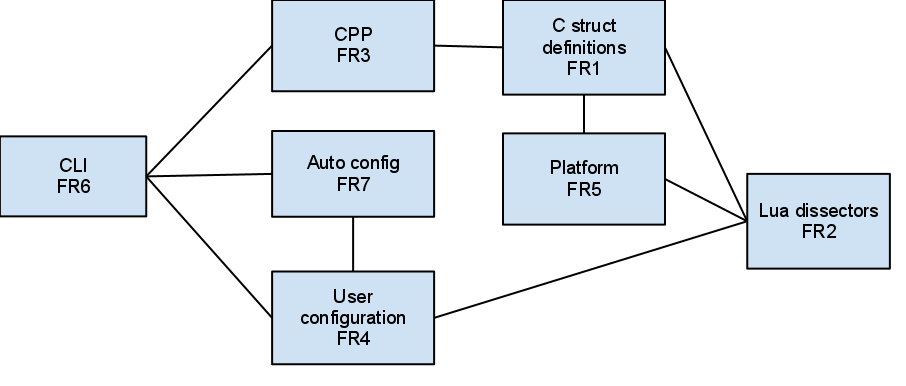
\includegraphics[width=\textwidth]{./planning/img/requirement_relationship}
	\caption{Relationship Between Requirements\label{fig:req:relationship}}
\end{figure}


%------------------
\section{Use Cases}
%------------------
\label{sec:req:usecases}
This sections contains use case diagrams for our two actors, and detailed
textual use cases for these diagrams.

\subsection{Actors}
%------------------
An actor specifies a role played by an external person or thing that interact
with our \gls{utility}. We have three types of actors to consider. First is the
primary actor, that uses the \gls{utility} to generate \glspl{dissector} from 
\Gls{c} header-files. A secondary actor is the user who configures the
\gls{utility} to change the output of it. Finally, we have an offstage actor, which
does not use our \gls{utility} himself, but uses the outputted \glspl{dissector} in \Gls{wireshark}.

We have defined two use case actors for our \gls{utility}. The customer has specified
that the offstage actor, called developer, is the most important actor.
\begin{description}
	\item[Developer] User of the generated \Gls{wireshark} \glspl{dissector}, offstage actor
	\item[Administrator] User and configurer of \gls{utility}, primary and secondary actor
\end{description}

\subsection{Use Case Diagrams}
%-----------------------------
\hyperref[fig:req:ucadm]{Figure \ref*{fig:req:ucadm}} shows the use case
diagram for the administrator, and \autoref{fig:req:ucdev} is the use case
diagram for the developer.
\begin{figure}[htbp]
	\center
	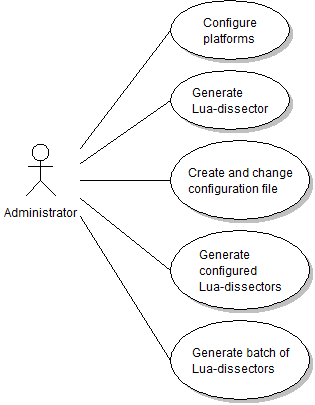
\includegraphics[width=0.6\textwidth]{./planning/img/uc_administrator}
	\caption{Use Case Diagram: Administrator\label{fig:req:ucadm}}
\end{figure}

\begin{figure}[htbp]
	\center
	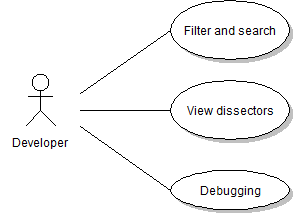
\includegraphics[width=0.6\textwidth]{./planning/img/uc_developer}
	\caption{Use Case Diagram: Developer\label{fig:req:ucdev}}
\end{figure}

\subsection{Textual Use Cases}
%-----------------------------
Here each of the use cases are described textually.

\begin{table}[htbp] \footnotesize \center
\caption{Filter and Search Textual Use Case\label{tab:textual:filterandsearch}}
\begin{tabularx}{\textwidth}{l X}
	\multicolumn{2}{c}{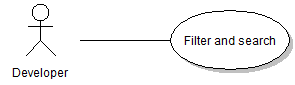
\includegraphics[scale=0.8]{./planning/img/uc_filterandsearch}} \\
	\toprule
	Element & Description\\
	\midrule
	Use case name & Filter and search on attributes\\
	Goal & The developer wants the correct set of results based on the search phrase \\
	Summary & The developer would like to filter and search on attributes in the packets displayed in Wireshark \\
	Preconditions & Wireshark need to be running with dissectors. \\
	Postconditions & Wireshark display the results.\\
	\midrule
	\multirow{3}{*}{Flow of Events} & 1. The developer selects the search field in Wireshark's GUI.  \\
	& 2. The user types in a search phrase. \\
	& 3. Wireshark will present the search results that match the query. \\
	\midrule
	Exceptions & None. \\
	\bottomrule
\end{tabularx}
\end{table}

\begin{table}[htbp] \footnotesize \center
\caption{View Dissector Textual Use Case\label{tab:textual:viewdissector}}
\begin{tabularx}{\textwidth}{l X}
	\multicolumn{2}{c}{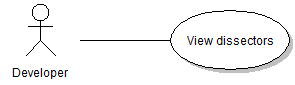
\includegraphics[scale=0.8]{./planning/img/uc_viewdissectors}} \\
	\toprule
	Element & Description\\
	\midrule
	Use case name & View the dissectors in Wireshark\\
	Goal & View structs correctly dissected in Wireshark\\
	Summary & The developer would like to dissect a structs and have the members and values displayed in Wireshark by using the dissectors in Wireshark's plugin folder.\\
	\multirow{2}{*}{Preconditions}& 1. The developer have Wireshark running with dissectors. \\
	& 2. The dissector for a struct will dissect it correctly, according to the initial internal structure of the struct. \\
	Postconditions & Wireshark display the struct with the correct structure and values.\\
	\midrule
	\multirow{3}{*}{Flow of Events} & 1. The developer selects a struct message in Wireshark. \\
	& 2. Wireshark calls the correct dissector and dissects the selected message. \\
	& 3. Wireshark displays the members and values of the selected message. \\
	\midrule
	Exceptions & 1. The correct dissector for a struct might not exist in Wireshark's plugin folder, making it impossible to dissect the message. \\
	\bottomrule
\end{tabularx}
\end{table}

\begin{table}[htbp] \footnotesize \center
\caption{Debugging Textual Use Case\label{tab:textual:debugging}}
\begin{tabularx}{\textwidth}{l X}
	\multicolumn{2}{c}{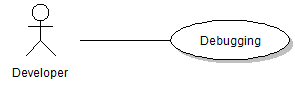
\includegraphics[scale=0.8]{./planning/img/uc_debugging}} \\
	\toprule
	Element & Description\\
	\midrule
	Use case name & Debugging\\
	Goal & The developer wants to debug inter-process communication.\\
	Summary & The developer wants to debug inter-process communication by using Wireshark extended by dissectors. \\
	\multirow{2}{*}{Preconditions} & 1. The developer have Wireshark running with dissectors.\\
	& 2. Wireshark have access to the packets sent between the processes that the developer wants to debug. \\
	Postconditions & Wireshark display the communication dissected.\\
	\midrule
	\multirow{3}{*}{Flow of Events} & 1. The developer selects the inter-process communication to debug. \\
	& 2. Wireshark calls the correct dissector and dissects the selected messages. \\
	& 3. The developer is able to debug the process communication by looking at the dissected messages. \\
	\midrule
	\multirow{2}{*}{Exceptions} & 1. The correct dissectors might not exist in Wireshark's plugin folder, making it impossible to dissect the messages. \\
	& 2. The inter-process communication might not consist of structs only, which Wireshark do not have capability of displaying. \\
	\bottomrule
\end{tabularx}
\end{table}

\begin{table}[htbp] \footnotesize \center
\caption{Configure Platforms Textual Use Case\label{tab:textual:configureplatforms}}
\begin{tabularx}{\textwidth}{l X}
	\multicolumn{2}{c}{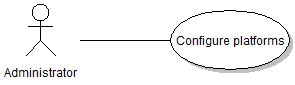
\includegraphics[scale=0.8]{./planning/img/uc_configureplatform}} \\
	\toprule
	Element & Description\\
	\midrule
	Use case name & Configure platforms\\
	Goal & Successfully configure the supported platforms.\\
	Summary & The administrator want to be able to configure the platforms that the utility supports. This includes adding, removing and editing supported platforms.\\
	Preconditions & The administrator must have access to the utility's platform module (the source code).\\
	Postconditions & The changes must be saved to the platform module.\\
	\midrule
	\multirow{3}{*}{Flow of Events} & 1. The administrator locates the platform module in the utility. \\
	& 2. The administrator make changes to the module to achieve the wanted support.\\
	& 3. The administrator saves the changes and exits. \\
	\midrule
	Exceptions & The changes made to the platform module were not of correct syntax. Leaving the utility defected. \\
	\bottomrule
\end{tabularx}
\end{table}

\begin{table}[htbp] \footnotesize \center
\caption{Generate Lua Dissector Textual Use Case\label{tab:textual:generatelua}}
\begin{tabularx}{\textwidth}{l X}
	\multicolumn{2}{c}{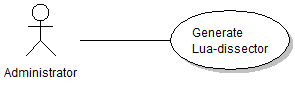
\includegraphics[scale=0.8]{./planning/img/uc_generatelua}} \\
	\toprule
	Element & Description\\
	\midrule
	Use case name & Generate Lua-dissector\\
	Goal & Successfully generate a Lua-dissector. \\
	Summary & The administrator wants to generate a Lua-dissector based on a header file. \\
	\multirow{2}{*}{Preconditions} & 1. The administrator have the utility and its dependent libraries installed.  \\
	& 2. The administrator have a header file, which a Lua-dissector shall be made of. \\
	Postconditions & The utility outputs the generated Lua-dissector to a default- or given output location. \\
	\midrule
	\multirow{3}{*}{Flow of Events} & 1. The Administrator feeds the utility with the header- and configuration file\\
	& 2. The utility generates a Lua-dissector based on the input. \\
	& 3. The utility outputs the Lua-dissector to a default- or given output location.\\
	\midrule
	\multirow{2}{*}{Exceptions} & 1. The header file might not be of correct syntax.\\
	& 2. The utility's dependencies might not be covered, resulting in a crash of the utility.\\
	\bottomrule
\end{tabularx}
\end{table}

\begin{table}[htbp] \footnotesize \center
\caption{Create and Change Configuration File Textual Use Case\label{tab:textual:configure}}
\begin{tabularx}{\textwidth}{l X}
	\multicolumn{2}{c}{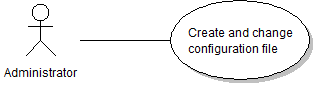
\includegraphics[scale=0.8]{./planning/img/uc_configurate}} \\
	\toprule
	Element & Description\\
	\midrule
	Use case name & Create and change configuration file\\
	Goal & Successfully create and/or change a configuration file. \\
	Summary & The administrator wants to create and/or change a configuration file. \\
	Preconditions & Create or find an existing configuration file \\
	Postconditions & Save the file.\\
	\midrule
	Flow of Events & The administrator changes the located file to get the wanted configuration.  \\
	\midrule
	Exceptions & The created or changed configuration file might not be of correct syntax. \\
	\bottomrule
\end{tabularx}
\end{table}

\begin{table}[htbp] \footnotesize \center
\caption{Generate Configured Lua Dissectors Textual Use Case\label{tab:textual:generateconfiglua}}
\begin{tabularx}{\textwidth}{l X}
	\multicolumn{2}{c}{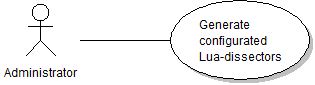
\includegraphics[scale=0.8]{./planning/img/uc_generateconfiglua}} \\
	\toprule
	Element & Description\\
	\midrule
	Use case name & Generate configured Lua-dissectors.\\
	Goal & Successfully generate a configured Lua-dissector. \\
	Summary & The administrator wants to generate a Lua-dissector from a header file with an associated configuration file. \\
	\multirow{2}{*}{Preconditions} & 1. The administrator have the utility and its dependent libraries installed.  \\
	& 2. The administrator have the header and configuration pair, which the Lua-dissector shall be made of. \\
	Postconditions & The utility outputs the generated Lua-dissector to a default- or given output location.\\
	\midrule
	\multirow{3}{*}{Flow of Events} & 1. The Administrator feeds the utility with the header- and configuration-file\\
	& 2. The utility generates a Lua-dissector based on the input. \\
	& 3. The utility outputs the Lua-dissector to a default- or given output location.\\
	\midrule
	\multirow{2}{*}{Exceptions} & 1. The header and/or configuration file might not be of correct syntax.\\
	& 2. The utility's dependencies might not be covered, resulting in a crash of the utility.\\
	\bottomrule
\end{tabularx}
\end{table}

\begin{table}[htbp] \footnotesize \center
\caption{Generate Batch of Lua Dissectors Textual Use Case\label{tab:textual:luabatch}}
\begin{tabularx}{\textwidth}{l X}
	\multicolumn{2}{c}{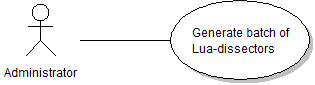
\includegraphics[scale=0.8]{./planning/img/uc_luabatch}} \\
	\toprule
	Element & Description\\
	\midrule
	Use case name & Generate batch of Lua-dissectors.\\
	Goal & Successfully create multiple Lua-dissectors. \\
	Summary & The administrator wants to process multiple header- and configuration-file pairs in one run of the utility. \\
	Preconditions & The administrator know the locations of all the files to parse. \\
	Postconditions & The utility outputs the generated Lua-dissectors to a default- or given output location.\\
	\midrule
	\multirow{3}{*}{Flow of Events} &  1. The administrator feeds the utility with the header- and configuration-files.\\
	& 2. The utility generates Lua-dissectors for all the input headers.	\\
	& 3. The utility outputs the Lua-dissectors to a default- or given output location.	\\
	\midrule
	\multirow{2}{*}{Exceptions} & 1. A header or configuration file might not be of correct syntax, which will make the utility skip that actual file and proceed with the rest of the files in the batch.\\
	& 2. The utility's dependencies might not be covered, resulting in a crash of the utility.\\
	\bottomrule
\end{tabularx}
\end{table}

\section{User Stories}
To make it easier to implement the requirements, there have been written user stories. The user stories describes how the requirements should be implemented, and was written in each sprint planning meeting. The user stories that are written can be found in the sprint design for each of the sprint. \autoref{tab:us:template} shows an template of an user story.

\begin{table}[htbp] \footnotesize \center
\caption{User Story Template\label{tab:us:template}}
\noindent\makebox[\textwidth]{%
\begin{tabularx}{1.2\textwidth}{l X}
\toprule
Header & Value \\
\midrule
ID & ID for the user stories, written like USxx. \\
Requirements & The requirement that the user story describes. \\
What & Description of what the user want to achieve.\\
How & Description of how the requirement should be implemented. \\
Result & What the result is after the implementation. \\
\bottomrule
\end{tabularx}}
\end{table}

